\documentclass[11pt, a4paper]{article}
\usepackage{hyperref}
\usepackage{graphicx}
\usepackage{enumitem}

\usepackage[T1]{fontenc}
\usepackage[font={footnotesize}]{caption}
\usepackage{wrapfig}
\usepackage{geometry}
\geometry{
 a4paper,
 total={170mm,257mm},
 left=35mm,
 right=30mm,
 top=40mm,
 bottom=15mm
 }

\usepackage{url}
\usepackage{hyperref}
\usepackage{indentfirst} % indent first paragraph
\usepackage[section]{placeins} % place figure inside section if declared in sec.
\setlength{\parindent}{-5mm}
\setlength{\parskip}{\baselineskip}%

\pagenumbering{gobble}

\newcommand{\bs}{\textbackslash}
% enumerate shortcuts \e
\def\e{\begingroup\catcode`\^^M=12 \xmymacro}
{\catcode`\^^M=12 %
 \gdef\xmymacro#1^^M{\begin{itemize}\item #1\end{itemize}\endgroup}%
}
\def\ee{\begingroup\catcode`\^^M=12 \xxmymacro}
{\catcode`\^^M=12 %
 \gdef\xxmymacro#1^^M{\begin{itemize}\item[]\begin{itemize}\item #1\end{itemize}\end{itemize}\endgroup}%
}
\def\eee{\begingroup\catcode`\^^M=12 \xxxmymacro}
{\catcode`\^^M=12 %
 \gdef\xxxmymacro#1^^M{\begin{itemize}\item[]\begin{itemize}\item[]\begin{itemize}\item #1\end{itemize}\end{itemize}\end{itemize}\endgroup}%
}

%\renewcommand{\texttildelow}[1][0pt]{%
%  \mathrel{\raisebox{#1}{\oldtexttildelow}}%
%}


\title{\vspace{-3cm}FiWi Würzburg Fortran Pipeline - Manual}
%\author{Lukas K. Schumann, \\\small{lukas\_kilian.schumann@stud-mail.uni-wuerzburg.de}}
\date{Stand: 03.2022}

\begin{document}

\maketitle

\bigskip\noindent


\vspace{-1cm}
\section{Installation}


Stelle sicher, dass SSH keys bereits generiert wurden. Dies wurde vermutlich schon erledit ist aber notwendig für weitere Schritte.
SSH keys befinden sich im Ordner \texttt{\%userprofile\%\bs.ssh} und können über den Konsolenbefehl \texttt{ssh-keygen} generiert werden, siehe Sec. \ref{sec:ssh}.

\begin{wrapfigure}{r}{0.55\linewidth}
    \centering
    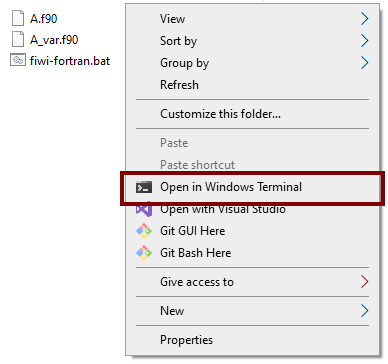
\includegraphics[width=0.65\linewidth]{./pics/2022-03-08_23-52.png}
    \caption{Terminal an diesem Ort öffnen}
    \vspace{-5em}
    \label{fig:install-1}
\end{wrapfigure}

Im Skript müssen können folgende Variablen gesetzt werden:
\e \texttt{REMOTEUSER} muss auf den eigenen Benutzeraccount gesetzt werden
\e \texttt{IPADDRESS} verweist auf den Koordinator Server und sollte in den meisten Fällen nicht geändert werden.

Anschließend kann das heruntergeladene Script mit \texttt{-{}-install} aufgerufen werden, siehe Fig.\ref{fig:install-1}.

Hier muss einmalig mit '\texttt{ja}' bzw. '\texttt{yes}' bestätigt werden, dass der Server in die Liste der bekannten Server aufgenommen werden soll.

\begin{figure}[h]
    \centering
    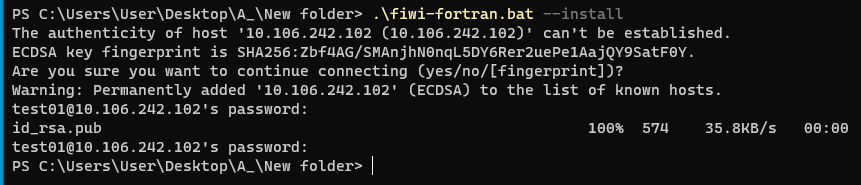
\includegraphics[width=1\linewidth]{./pics/2022-03-08_23-57.png}
    \caption{So kann die Installation gestartet werden.}
    \label{fig:install-2}
\end{figure}

Anschließend muss zweimal das Passwort eingegeben werden, siehe Fig.\ref{fig:install-2} für einen beispielhaften Ablauf.


%\begin{figure}[b]
%    \centering
%    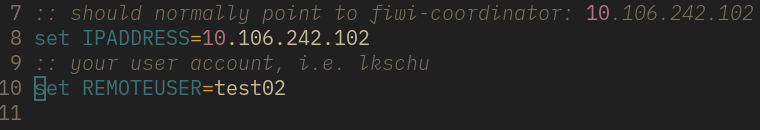
\includegraphics[width=0.9\linewidth]{./pics/2022-03-08_16-35.png}
%    \caption{\texttt{REMOTEUSER} Variable in fiwi-fortran.bat bzw. fiwi-fortan.sh}
%    \label{fig:remoteuser}
%\end{figure}


%\begin{figure}[b]
%    \centering
%    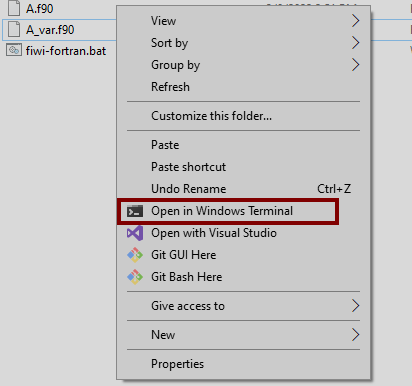
\includegraphics[width=0.45\linewidth]{./pics/2022-03-08_16-44.png}
%    \caption{Terminal an diesem Ort öffnen}
%    \label{fig:install-1}
%\end{figure}

\clearpage


\section{Nutzung}

\begin{figure}[htb!]
    \centering
    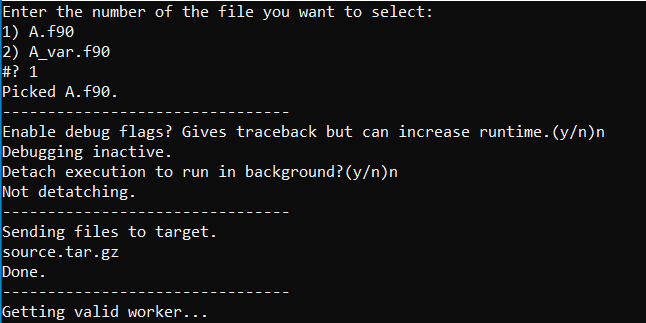
\includegraphics[width=0.7\linewidth]{./pics/2022-03-08_23-59_1.png}
    \caption{Beispielhafter Ablauf (1/2)}
    %\vspace{-5em}
    \label{fig:usage}
\end{figure}

Zur Nutzung das Programm in den Projektordner kopieren und mit Doppelklick starten.

Es folgt eine Auflistung aller im aktuellen Verzeichnis befindenden .f90 Dateien.
Die auszuführende Datei kann einfach durch Eingabe der entsprechenden Zahl bestätigt werden, siehe Fig.\ref{fig:usage}.

Weitere benötigte Dateien, wie zb. für Parameter/Variablen werden automatisch mit übermittelt, sofern sie sich im selben Verzeichnis befinden und auch mit .f90 enden.

Es folgt die Frage ob '\emph{debug flags}' verwendet werden sollen.
Dies führt zu einer erhöhten Laufzeit, meist ca. 10-30\%, gibt jedoch bei den meisten Fehlern traceback, aus dem Zeilennummern der Quelldatei auslesbar sind, die für den Fehler verantwortlich sind.
Mit '\texttt{y}' bestätigen bzw. mit '\texttt{n}' ablehnen.

\begin{figure}[h]
    \centering
    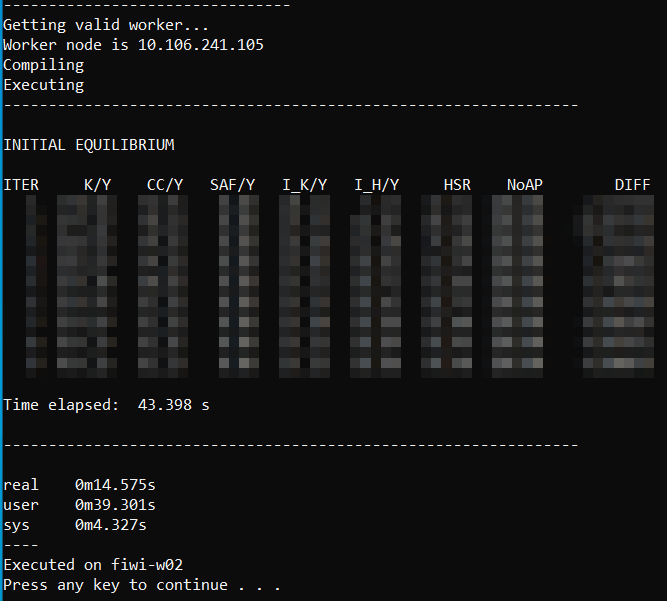
\includegraphics[width=0.7\linewidth]{./pics/2022-03-09_00-05.png}
    \caption{Beispielhafter Ablauf (2/2)}
    %\vspace{-5em}
    \label{fig:usage-full}
\end{figure}

Analog wird gefragt ob die Ergebnisse unmittelbar, über das Konsolenfenster verfügbar sein sollen - und damit abbrechen würde falls die Internetverbindung abbricht, oder das Programm in einen Hintergrund Prozess des Servers geforkt werden soll.

In beiden Fällen sind Ergebnisse über die Website auf \texttt{https://10.106.242.102/\raisebox{0.5ex}{\texttildelow}<username>} aufrufbar, wobei '\texttt{\raisebox{0.5ex}{\texttildelow}}' nicht vergessen werden darf!

Bei erstmaligem öffnen wird der Webbrowser eine Warnung mit dem Namen \texttt{SEC\_ERROR\_UNKNOWN\_ISSUER}, \texttt{ERR\_CERT\_AUTHORITY\_INVALID}, oder ähnlich presentieren, da das Zertifikat selbst signiert wurde.
Hier bitte einmal auf \emph{advanced} klicken und bestätigen.
siehe Fig.\ref{fig:web-1}.

\begin{figure}[h]
    \centering
    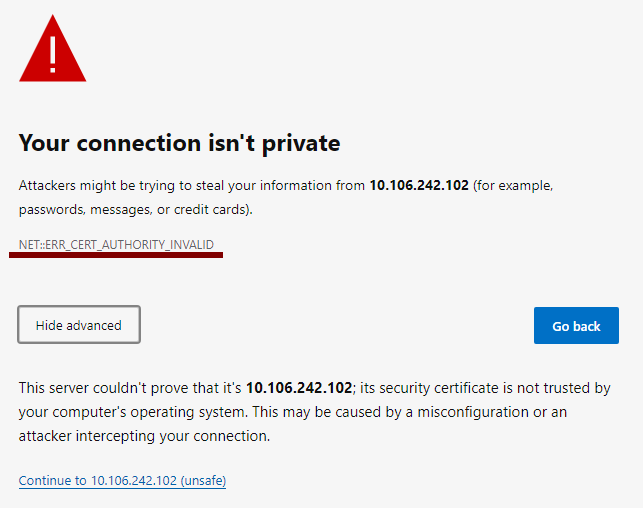
\includegraphics[width=0.7\linewidth]{./pics/2022-03-09_01-03_1.png}
    \caption{Ausnahme für Website hinzufügen}
    %\vspace{-5em}
    \label{fig:web-1}
\end{figure}

Nach der Eingabe der Benutzerdaten ist oben die aktuelle Auslastung aller verbundenen Maschinen, sowie im Zentrum die Ausgabe der letzten max. 7 Programme in Ordnern gelistet, deren Namen dem Startdatum und Zeitpunkt entsprechen.

Die Datei \texttt{console.txt}, die sich in jedem Ordner finden lässt, enthält die umgeleitete Standardausgabe, d.h. das, was sonst in der Konsole lesbar gewesen wäre.

\begin{figure}[h]
    \centering
    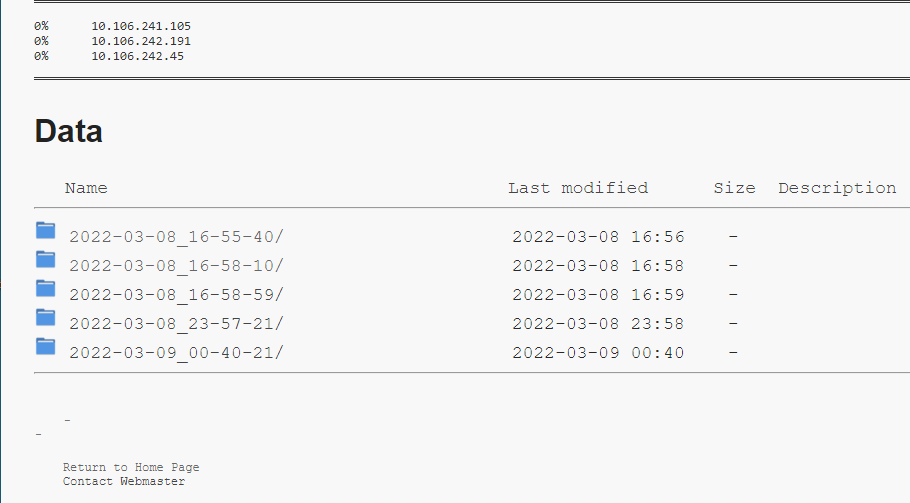
\includegraphics[width=0.7\linewidth]{./pics/2022-03-09_01-18.png}
    \caption{Ausnahme für Website hinzufügen}
    %\vspace{-5em}
    \label{fig:web-1}
\end{figure}

Weitere Funktionalitäten, wie das beenden fälschlich gestarteter Programme mittels \texttt{--kill}, sowie das Auflisten und Verunterladen älterer Ergebnisse mittels \texttt{--ls, --get} folgt die nächsten Tage.


\section{Problemlösung}

\subsection{Keine SSH keys vorhanden}\label{sec:ssh}
Konsole öffnen, den Befehl \texttt{ssh-keygen} ausführen und nächste Eingaben alle leer mit \texttt{<enter>} bestätigen um einen SSH key im default Speicherort ohne Passwort zu erstellen, siehe Fig. \ref{fig:ssh}.

\textbf{Achtung:} Sollten bereits SSH keys vorhanden sein werden und sollten diese nicht überschrieben, esseiden es wird explizit bestätigt.

\begin{figure}[h]
    \centering
    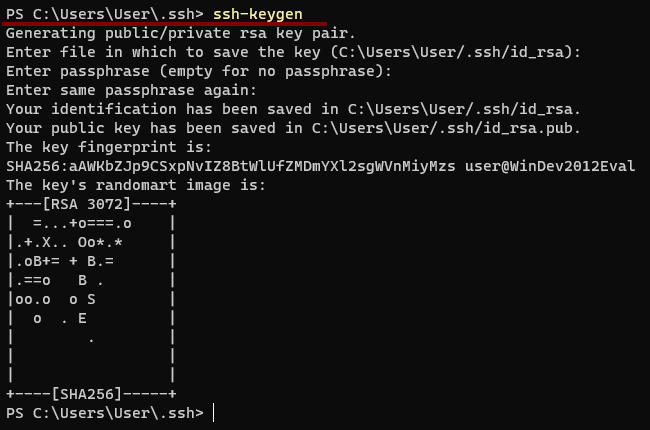
\includegraphics[width=0.7\linewidth]{./pics/2022-03-09_00-17.png}
    \caption{SSH keys generieren}
    %\vspace{-5em}
    \label{fig:ssh}
\end{figure}

\subsection{Fehlende Berechtigungen unter MacOS oder Linux}
Lässt sich das Script nicht starten müssen möglicherweise Berechtigungen überprüft werden.

Hierfür ein Konsolenfenster öffnen und mit folgendem Befehl Ausführberechtigungen erteilen: \newline\texttt{chmod +x "/pfad/zu/meiner datei.sh"}

Unter MacOS könnte es zusätzlich noch notwendig sein eine sog. erweiterte Dateieigenschaft zu entfernen.
Diese sind mittels: \newline\texttt{xattr "/pfad/zu/meiner datei.sh"}\newline einsehbar, wobei bei Bedarf \emph{com.apple.quarantine} mittels: \newline\texttt{xattr -d com.apple.quarantine "/pfad/zu/meiner datei.sh"}\newline entfernt werden kann.


\section{Kontakt}

Fragen, Fehlermeldungen, Ergänzungen und Anregungen können gerne an \underline{\href{mailto:lukas_kilian.schumann@stud-mail.uni-wuerzburg.de}{Lukas K. Schumann}} gesendet werden.

\end{document}

